
\documentclass{mcmthesis}
\mcmsetup{CTeX = false,   % 使用 CTeX 套装时,设置为 true
        tcn = 77281, problem = D,
        sheet = true, titleinsheet = true, keywordsinsheet = true,
        titlepage = true, abstract = true}
\usepackage{palatino}

\usepackage{float}


% 添加首行缩进,两个字符
\usepackage{indentfirst}
\setlength{\parindent}{2em}

\title{Driving(or Flying) On Electric}
\date{\today}
\begin{document}
\begin{abstract}

This paper mainly focuses on two aspects about charging stations, location and convenience, with the aim of formulating relevant policies to support the full adoption of electric vehicles.

We compare the Super Charger and the Destiny Charger of Telsla. Making use of the existing data of every charger's location and its stalls number, we plot the Voronoi Map, which indicates how the super charger stations are distributed solely across the USA highway and metropolises.

We search for the data concerning the number of USA EVs plus charging stations,and plot the numbers and their rate. We conclude that Tesla is on track to allow a complete switch to all-electric in the US.

Nowadays, there emerge various high-tech transportation modes such as rapid battery-swap stations for electric cars,car-share and ride-share services, self-driving cars, and even flying cars and a Hyper-loop.They will either accelarate the development of EV via shortening the charge time, reduce our bills in transportation, or speed up the public transport, etc. 


%
%Summary Sheet: The summary is an essential part of your MCM/ICM paper. 
%The judges place considerable weight on the summary, 
%and winning papers are often distinguished from other papers based on the quality of the summary.
%
%To write a good summary, imagine that a reader will choose whether to read the body of the paper based on your summary: 
%Your concise presentation in the summary should inspire a reader to learn about the details of your work. 
%Thus, a summary should clearly describe your approach to the problem and, most prominently, your most important conclusions.  
%Summaries that are mere restatements of the contest problem, or are a cut-and-paste boilerplate from the Introduction are generally considered to be weak.
%
%Besides the summary sheet as described each paper should contain the following sections:
%
%\begin{itemize}
%\item Restatement and clarification of the problem: State in your own words what you are going to do.
%\item Explain assumptions and rationale/justification: Emphasize the assumptions that bear on the problem. Clearly list all variables used in your model.
%\item Include your model design and justification for type model used or developed.
%\item Describe model testing and sensitivity analysis, including error analysis, etc.
%\item Discuss the strengths and weaknesses of your model or approach.
%\end{itemize}

\begin{keywords}
Electric Vehicals;  Charging Station Location
\end{keywords}

\end{abstract}
\maketitle
\section{Introduction}
With the rapid development of the automobile industry, the problems caused by automobiles such as environmental pollution and energy shortage have become increasingly prominent. In order to maintain the sustainable development of the national economy and protect the human living environment and energy supply, electric vehicles are gradually being favored by people for their environmental protection performance.
   
   However, the migration from gasoline and diesel cars to electric vehicles is not simple and can`t happen overnight. The challenge is how to design the distribution of charging stations, knowing that location and convenience are crucial to early adopters' feelings and whether they can become mainstream.
   
   Therefore, this paper mainly focuses on the two aspects of location and convenience to formulate relevant policies to support the full adoption of electric vehicles.

Here are the compare of Super Charger and Destiny Charger:

\begin{table}[!htbp]
\centering
\begin{tabular}{|c|c|c|}
\hline
 &Super Charger&Destiny Charger \\
\hline
cost&1000k&50k\\
\hline
price& 1.8RMB/kWh& 1.0RMB/kWh\\
\hline
time& 30min~1.5h& 6h\\
\hline
method&FAST &SLOW \\
\hline
\end{tabular}
\caption{Compare}
\end{table}

\begin{figure}[htbp]
\small
\centering
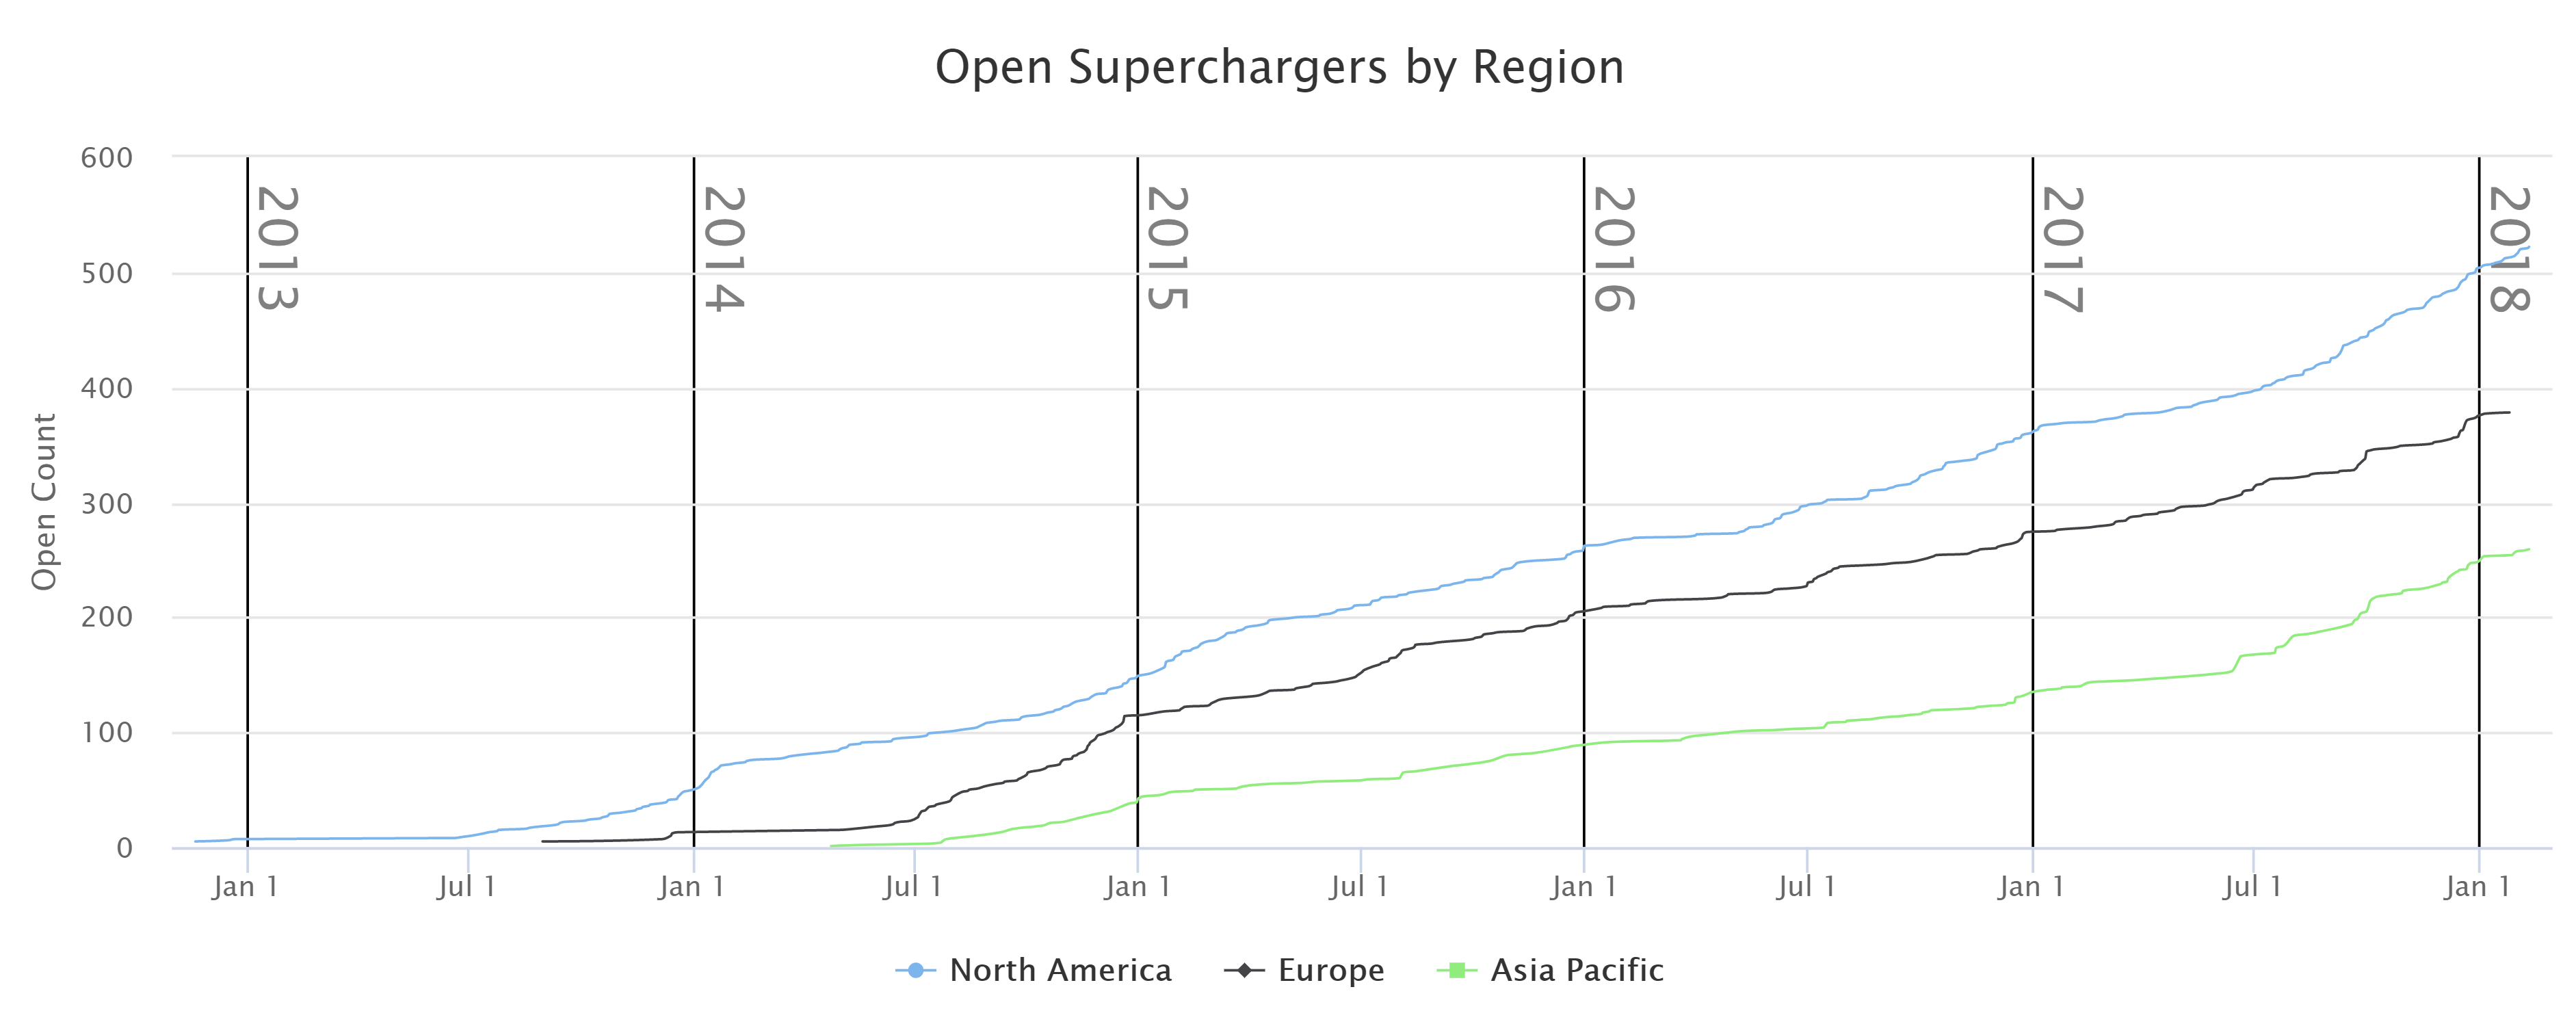
\includegraphics[width=16cm]{regions.png}
\caption{Open Superchargers By Regions} 
\end{figure}


\begin{figure}[htbp]
\small
\centering
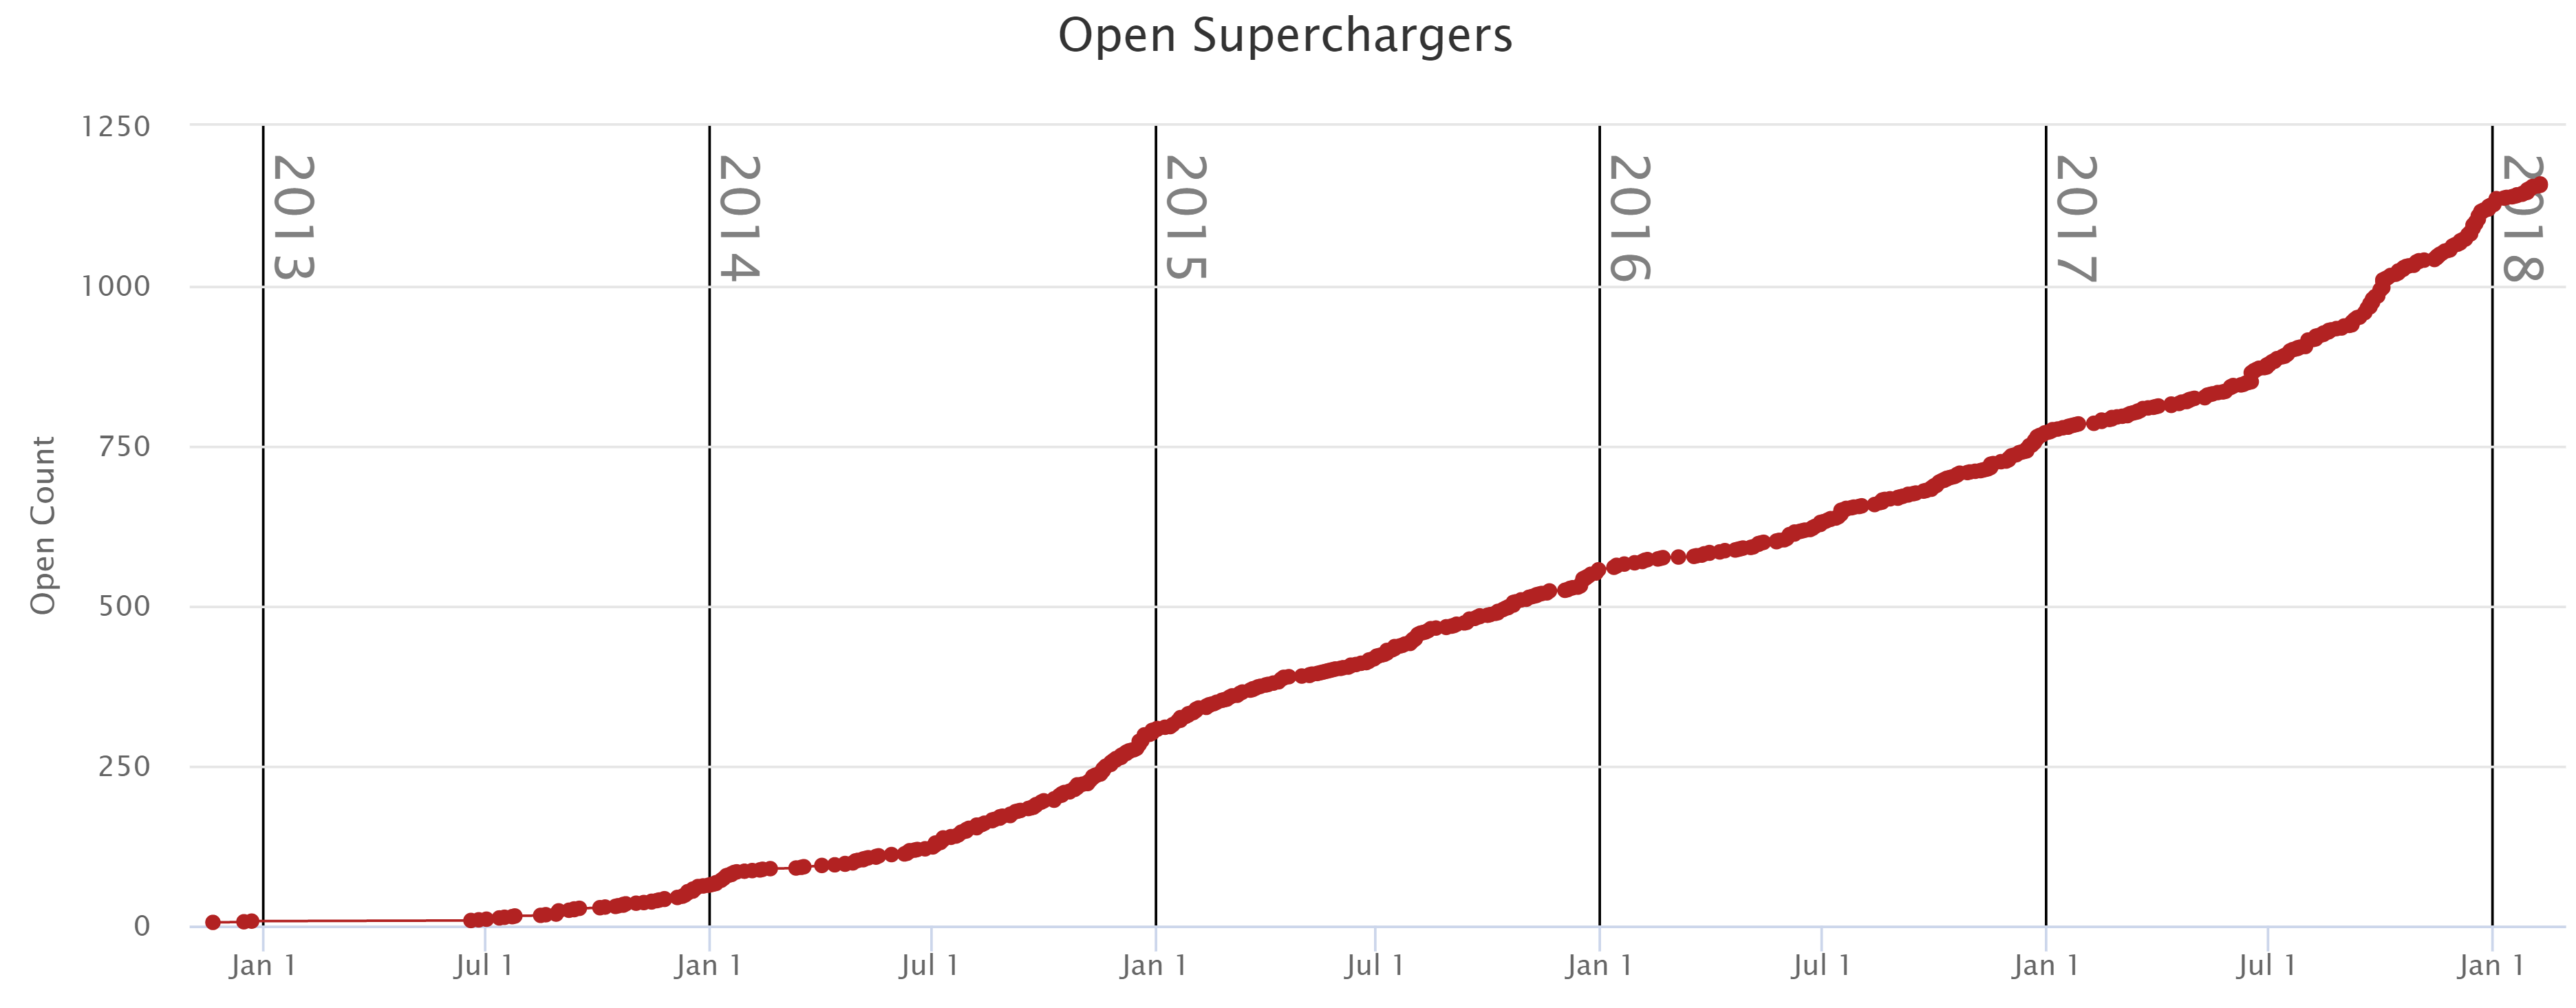
\includegraphics[width=16cm]{open.png}
\caption{Open Superchargers} 
\end{figure}


\begin{figure}[htbp]
\small
\centering
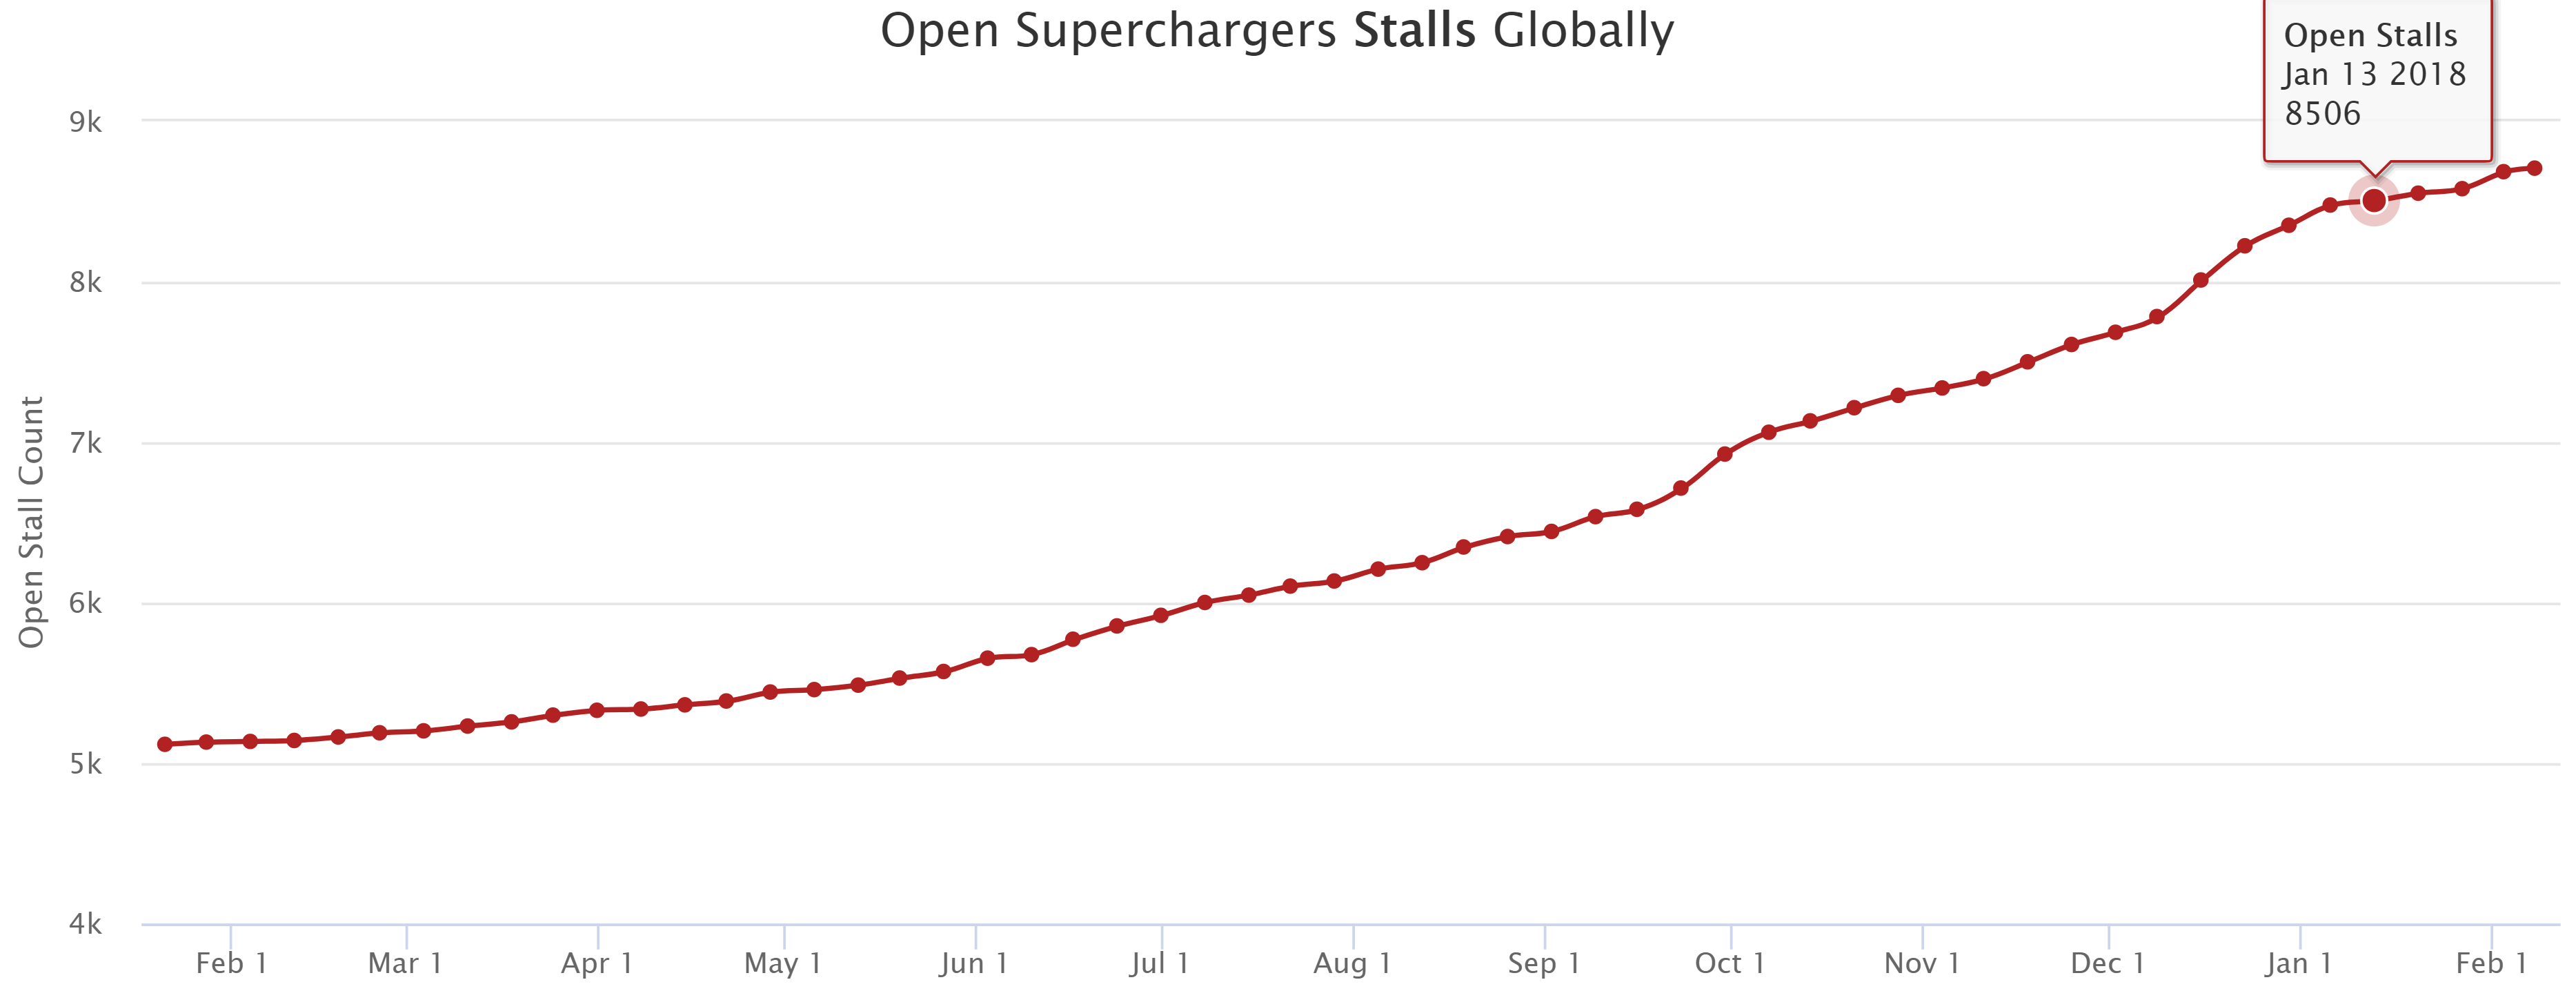
\includegraphics[width=16cm]{stall.png}
\caption{Open Superchargers Stall Globally} 
\end{figure}


\section{Analysis of the Problem}

\subsection {Location Model} 

 Let's consider such a transportation network, in which each electric vehicle is driven from a starting point to a destination. Due to the limits of its maximum battery capacity and mileage, vehicles must be charged on the way, or it can’t finish the whole trip. It is necessary to build sufficient charging stations on the road to meet charging requirements. This article introduces a new factor , the service capacity,  which refers to the amount of electricity one station can provide within a day.  In this article, service capacity is divided into two parts, which are divided into the number of charged piles and the electricity distribution of a charging station.

Our model meets the following conditions. First, the vehicle reaches the destination along the shortest route of the road. Second, the maximum driving range  of a vehicle is a constant number; The electric power dissipation and filling capacity of the vehicle has a linear relationship with the driving distance. Third, the car is not required to be fully charged, as long as the whole trip can be completed. Each motor vehicle can start with a half of the total charge.

\begin{figure}[htbp]
\small
\centering
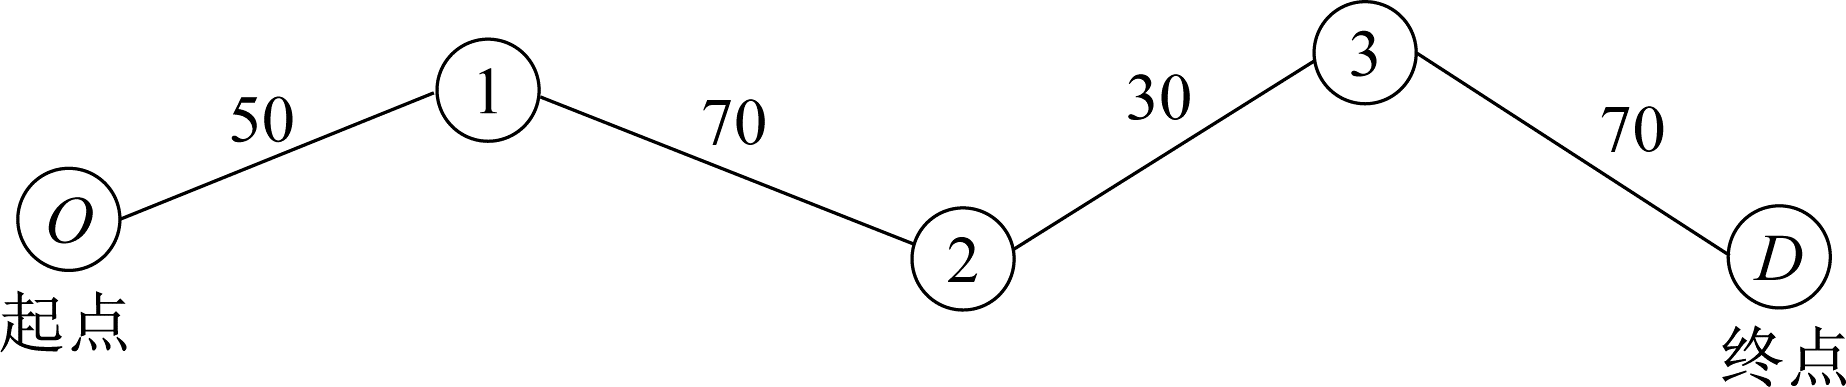
\includegraphics[width=12cm]{OD.png}
\caption{O-D Model} 
\end{figure}


\section{Task 1}

First, let's explore the current U.S. Tesla charging network. Tesla currently offers two types of charging stations


\begin{itemize}
\item destination charging designed for charging for several hours at a time or even overnight.
\item supercharging designed for longer road trips to provide up to 170 miles of range in as little as 30 minutes of charging.
\end{itemize}

In order to study whether Tesla is on an all-electric road, we use matlab to get the following figure based on the relevant database.

\begin{figure}[H]
\small
\centering
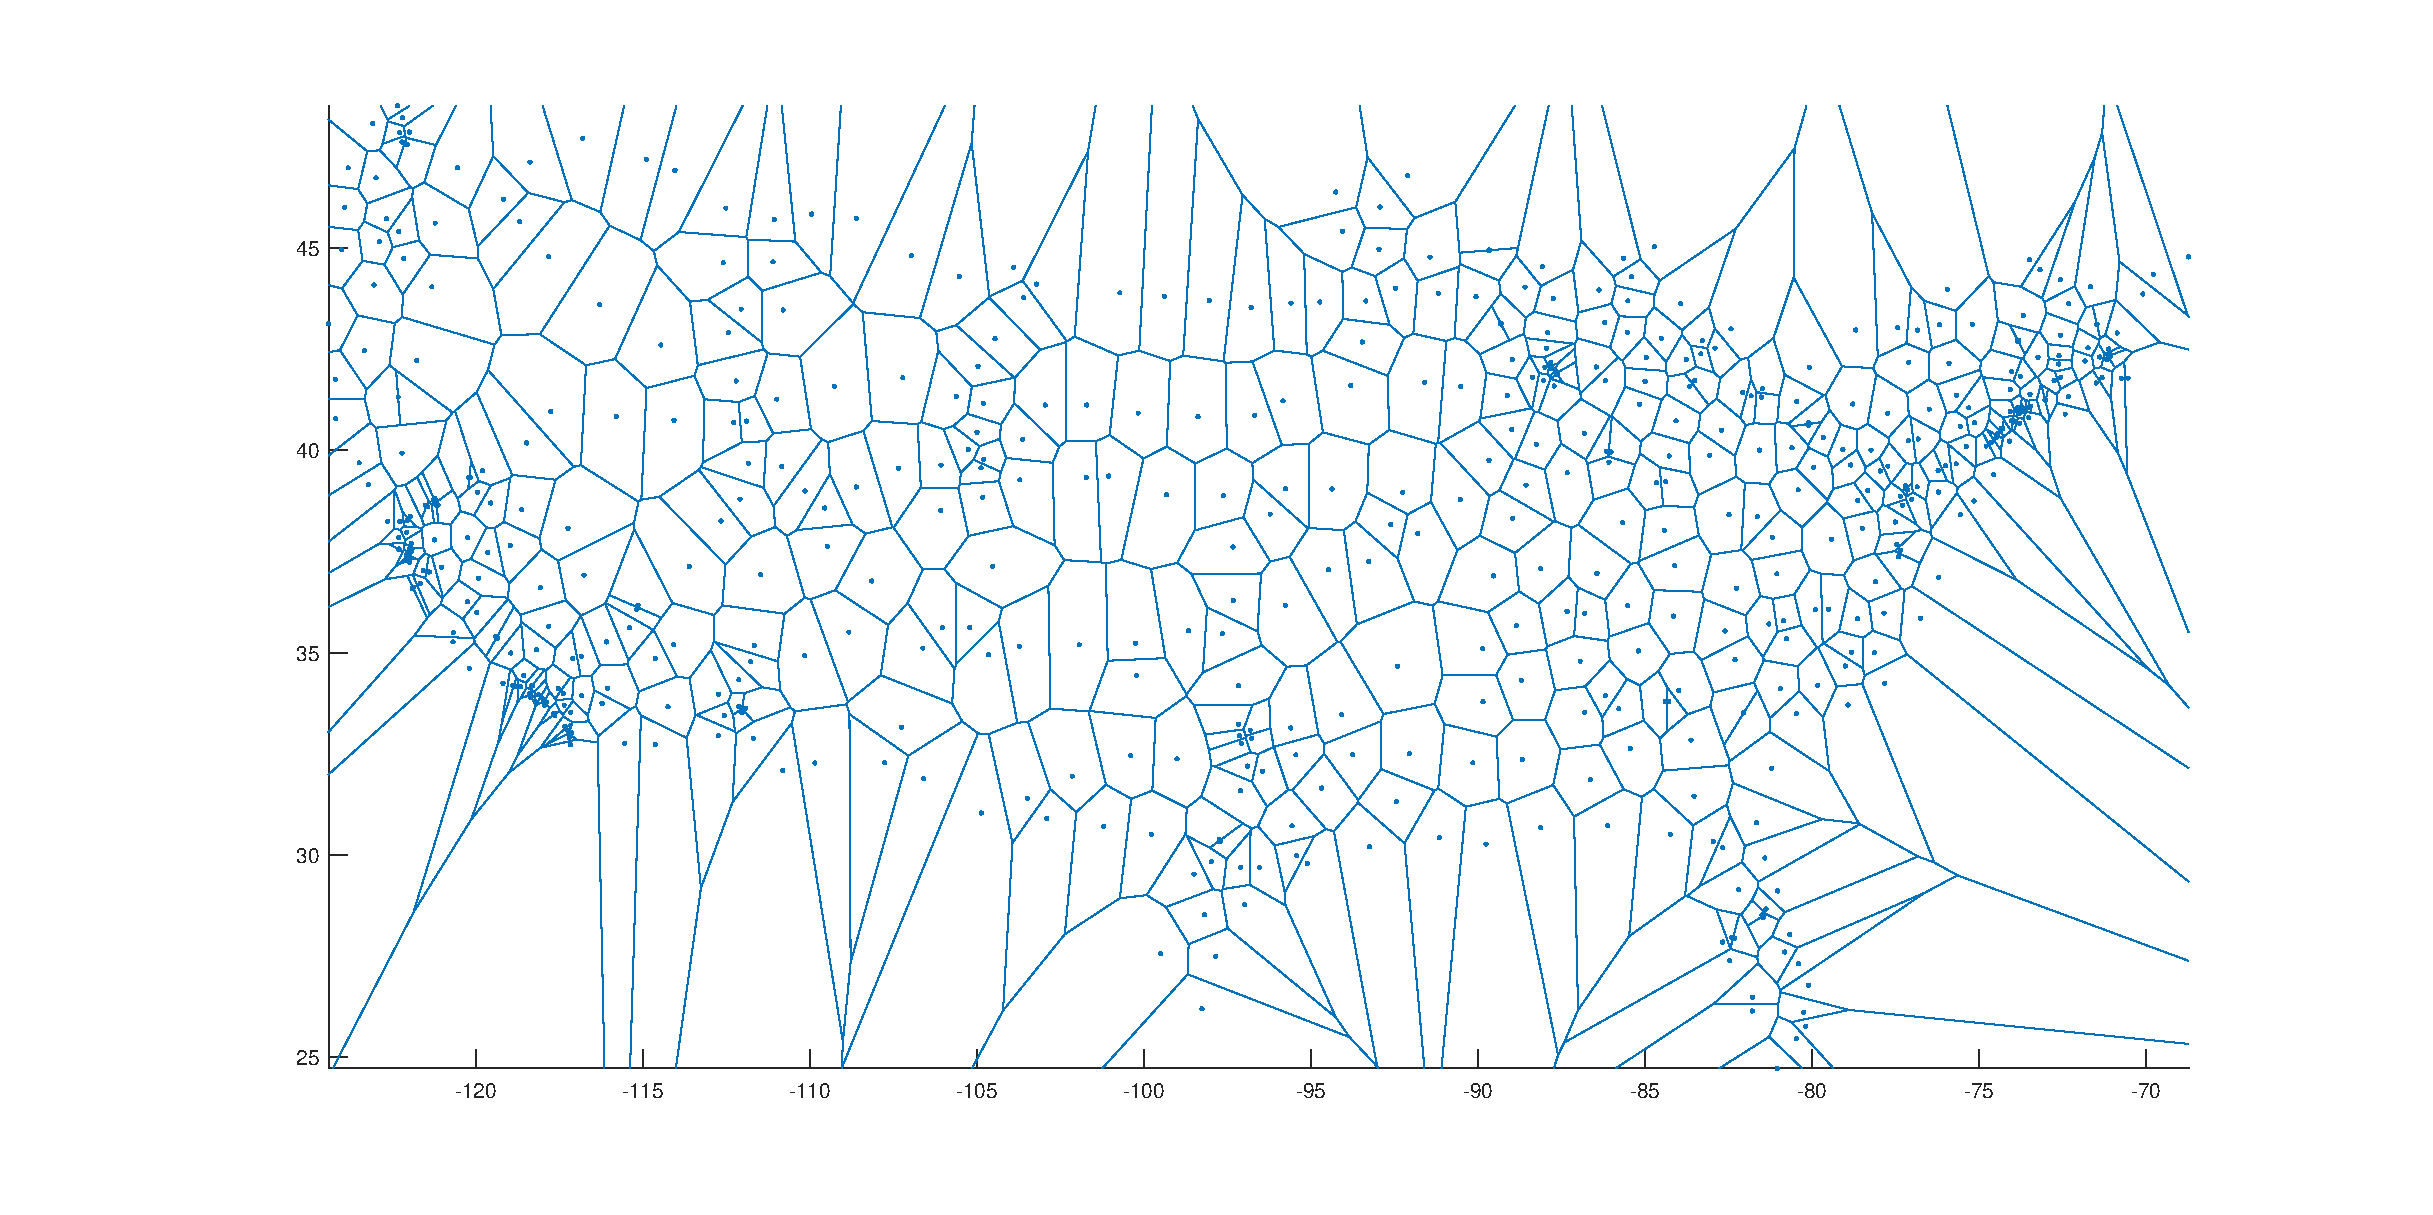
\includegraphics[width=16cm]{USAVoronoiMap.eps}
\caption{USA Voronoi Map} 
\end{figure}

\begin{figure}[htbp]
\small
\centering
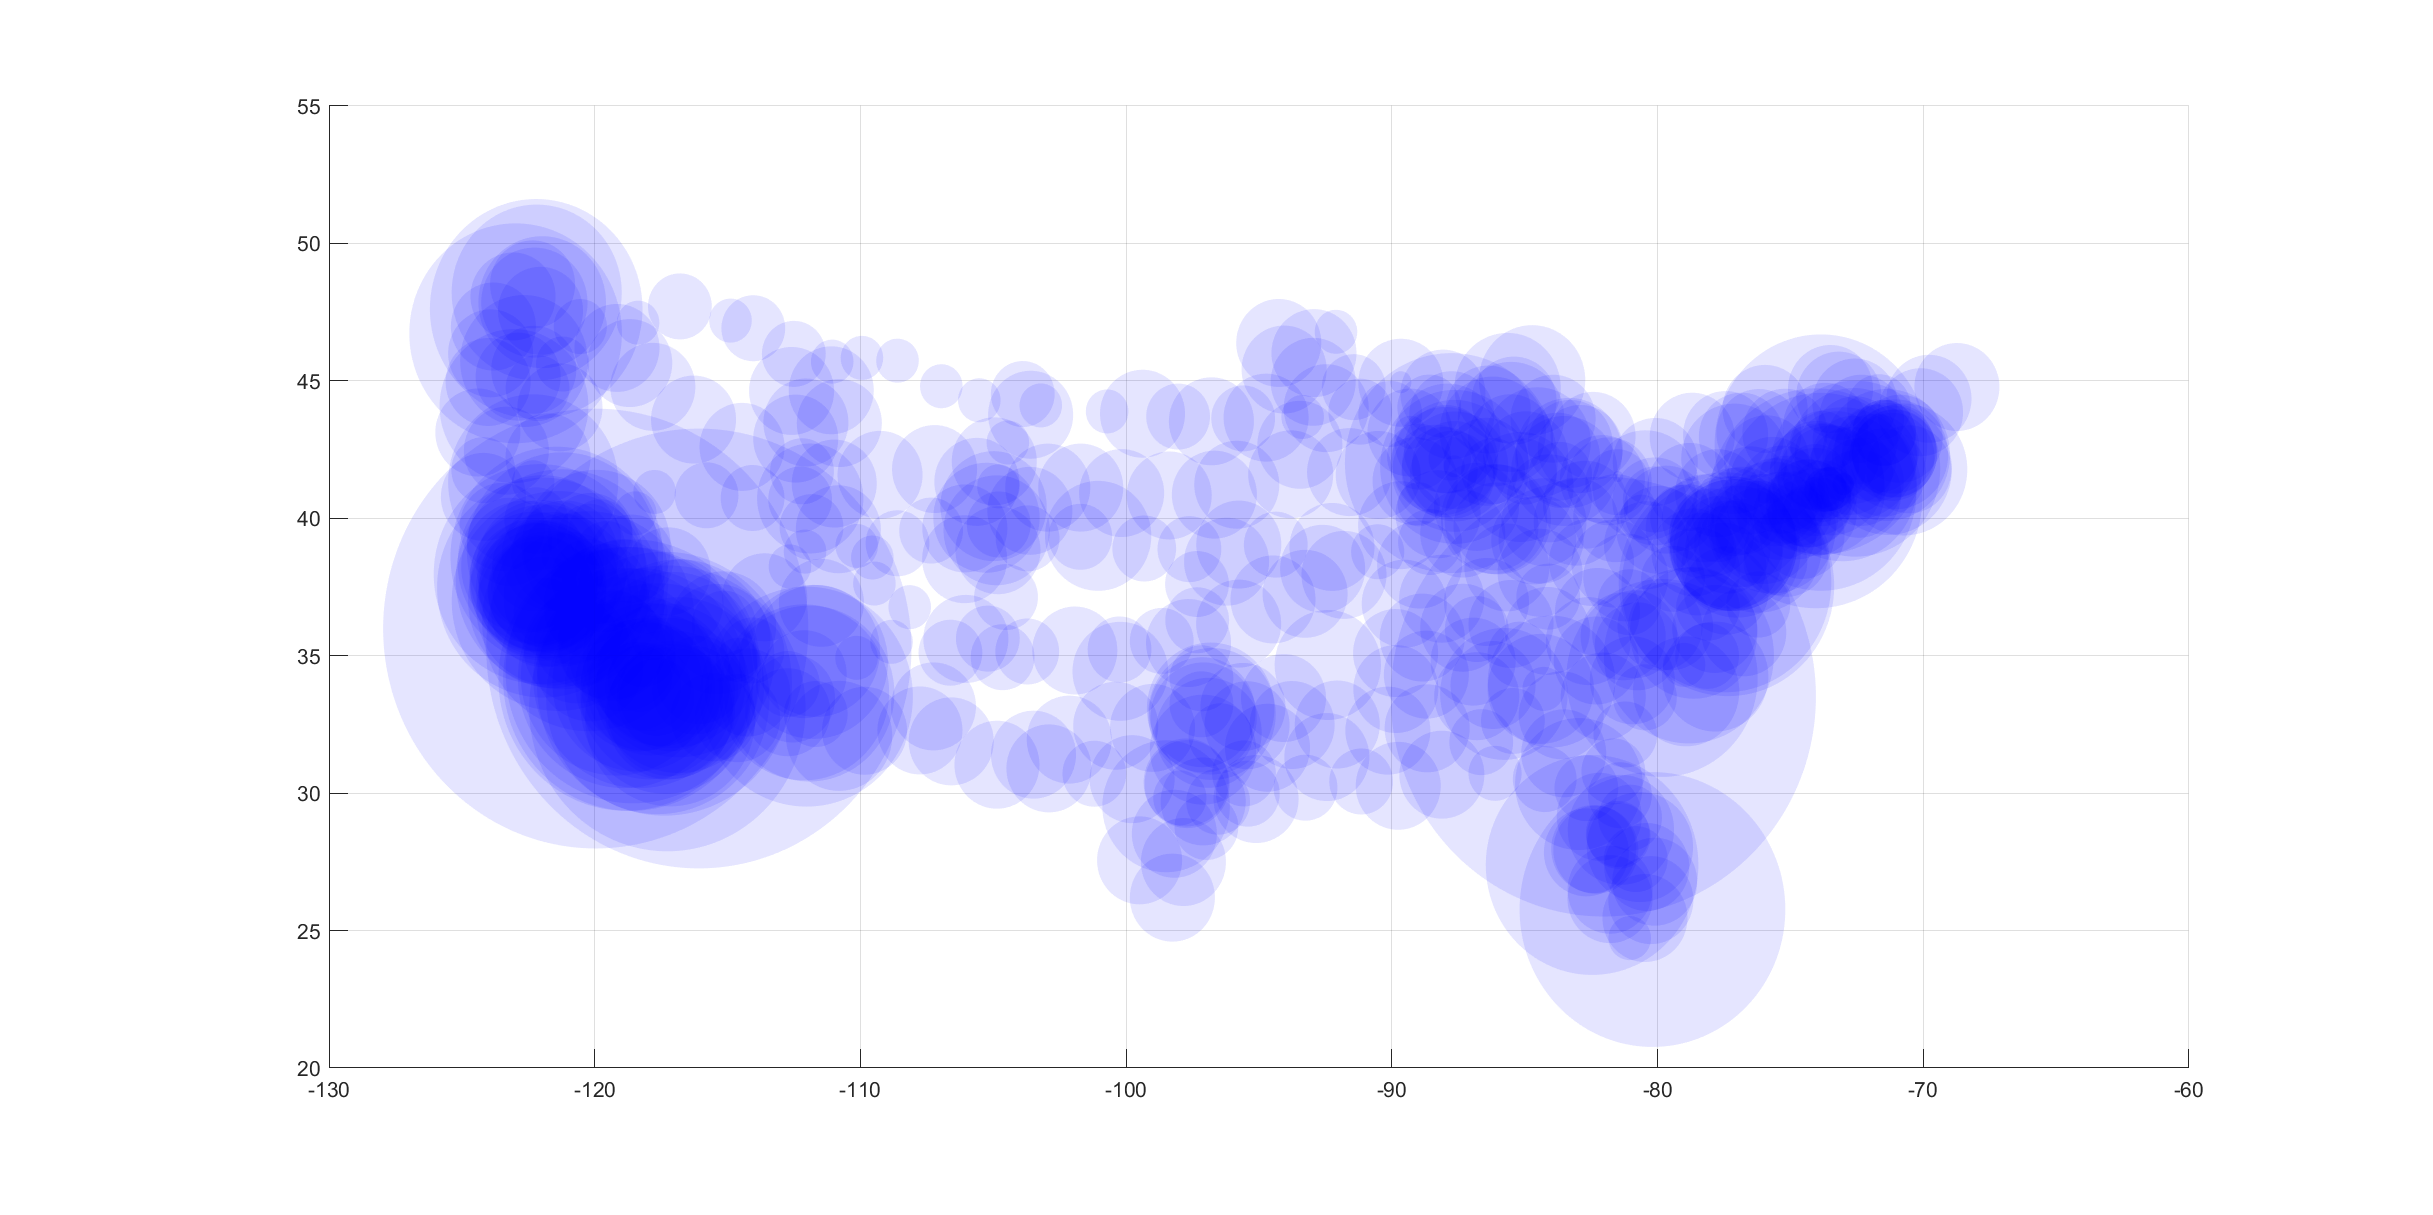
\includegraphics[width=18cm]{circular.eps}
\caption{USA Circular Map} 
\end{figure}


In our understanding, this issue mainly involves two angles:

\begin{itemize}
\item Comparison of vehicle sales and electric vehicle growth
\item The changes of Charging pile number whether can keep up with the sales of vehicles
\end{itemize}


It can be seen from the trend of two curves that the number of charging poles can keep up with the number of electric vehicles.


\begin{figure}[htbp]
\small
\centering
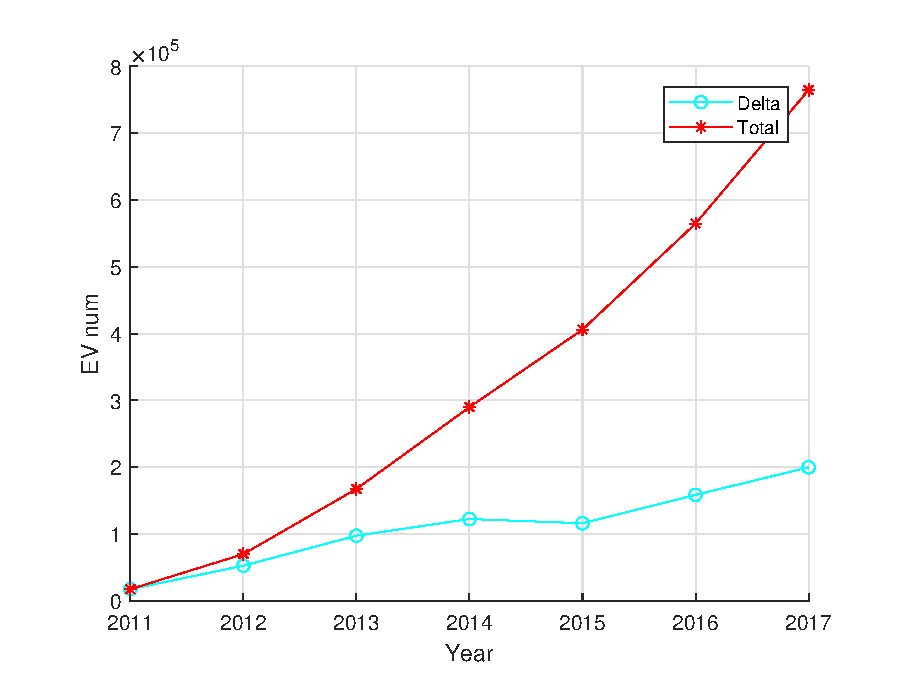
\includegraphics[width=14cm]{EVnum.eps}
\caption{EVnum} 
\end{figure}

\begin{figure}[htbp]
\small
\centering
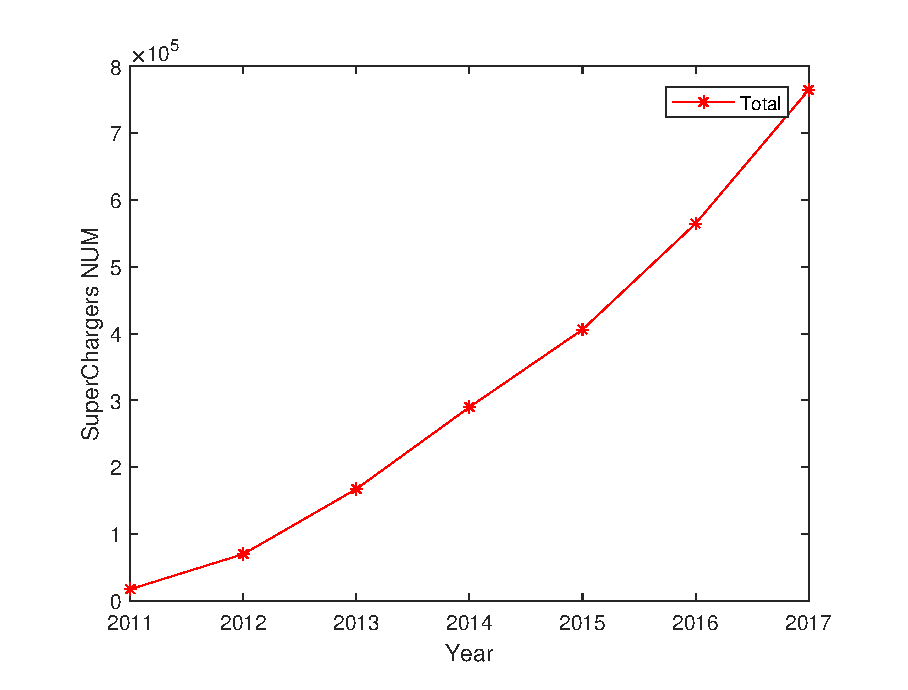
\includegraphics[width=14cm]{Superchargers.eps}
\caption{Super chargers} 
\end{figure}


\begin{figure}[H]
\small
\centering
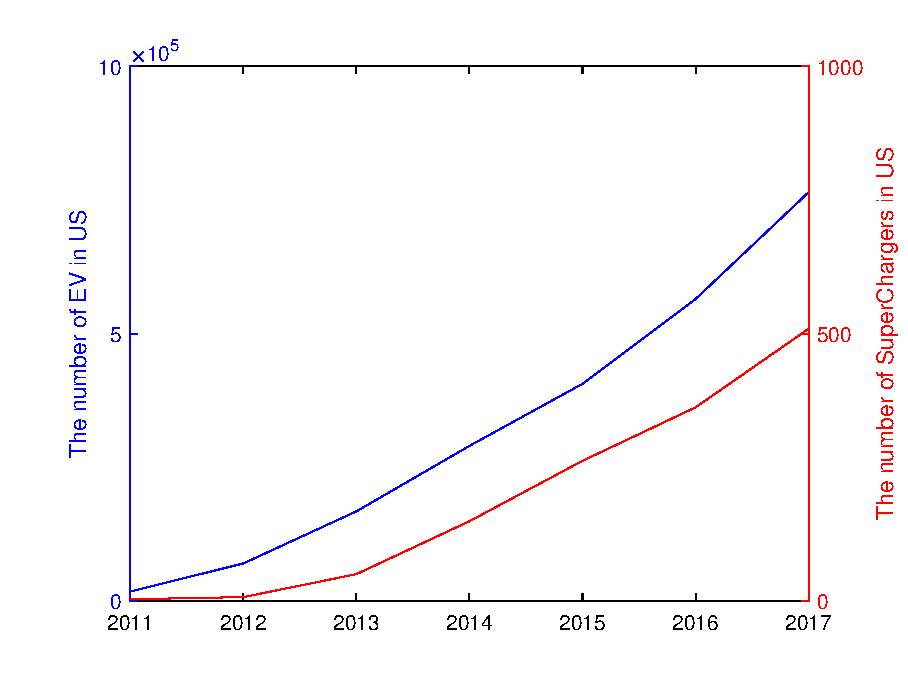
\includegraphics[width=14cm]{EVandChargers.eps}
\caption{EV and Chargers} 
\end{figure}

\section{Task 2}
We choose South Korea to analyse.
\begin{figure}[H]
\small
\centering
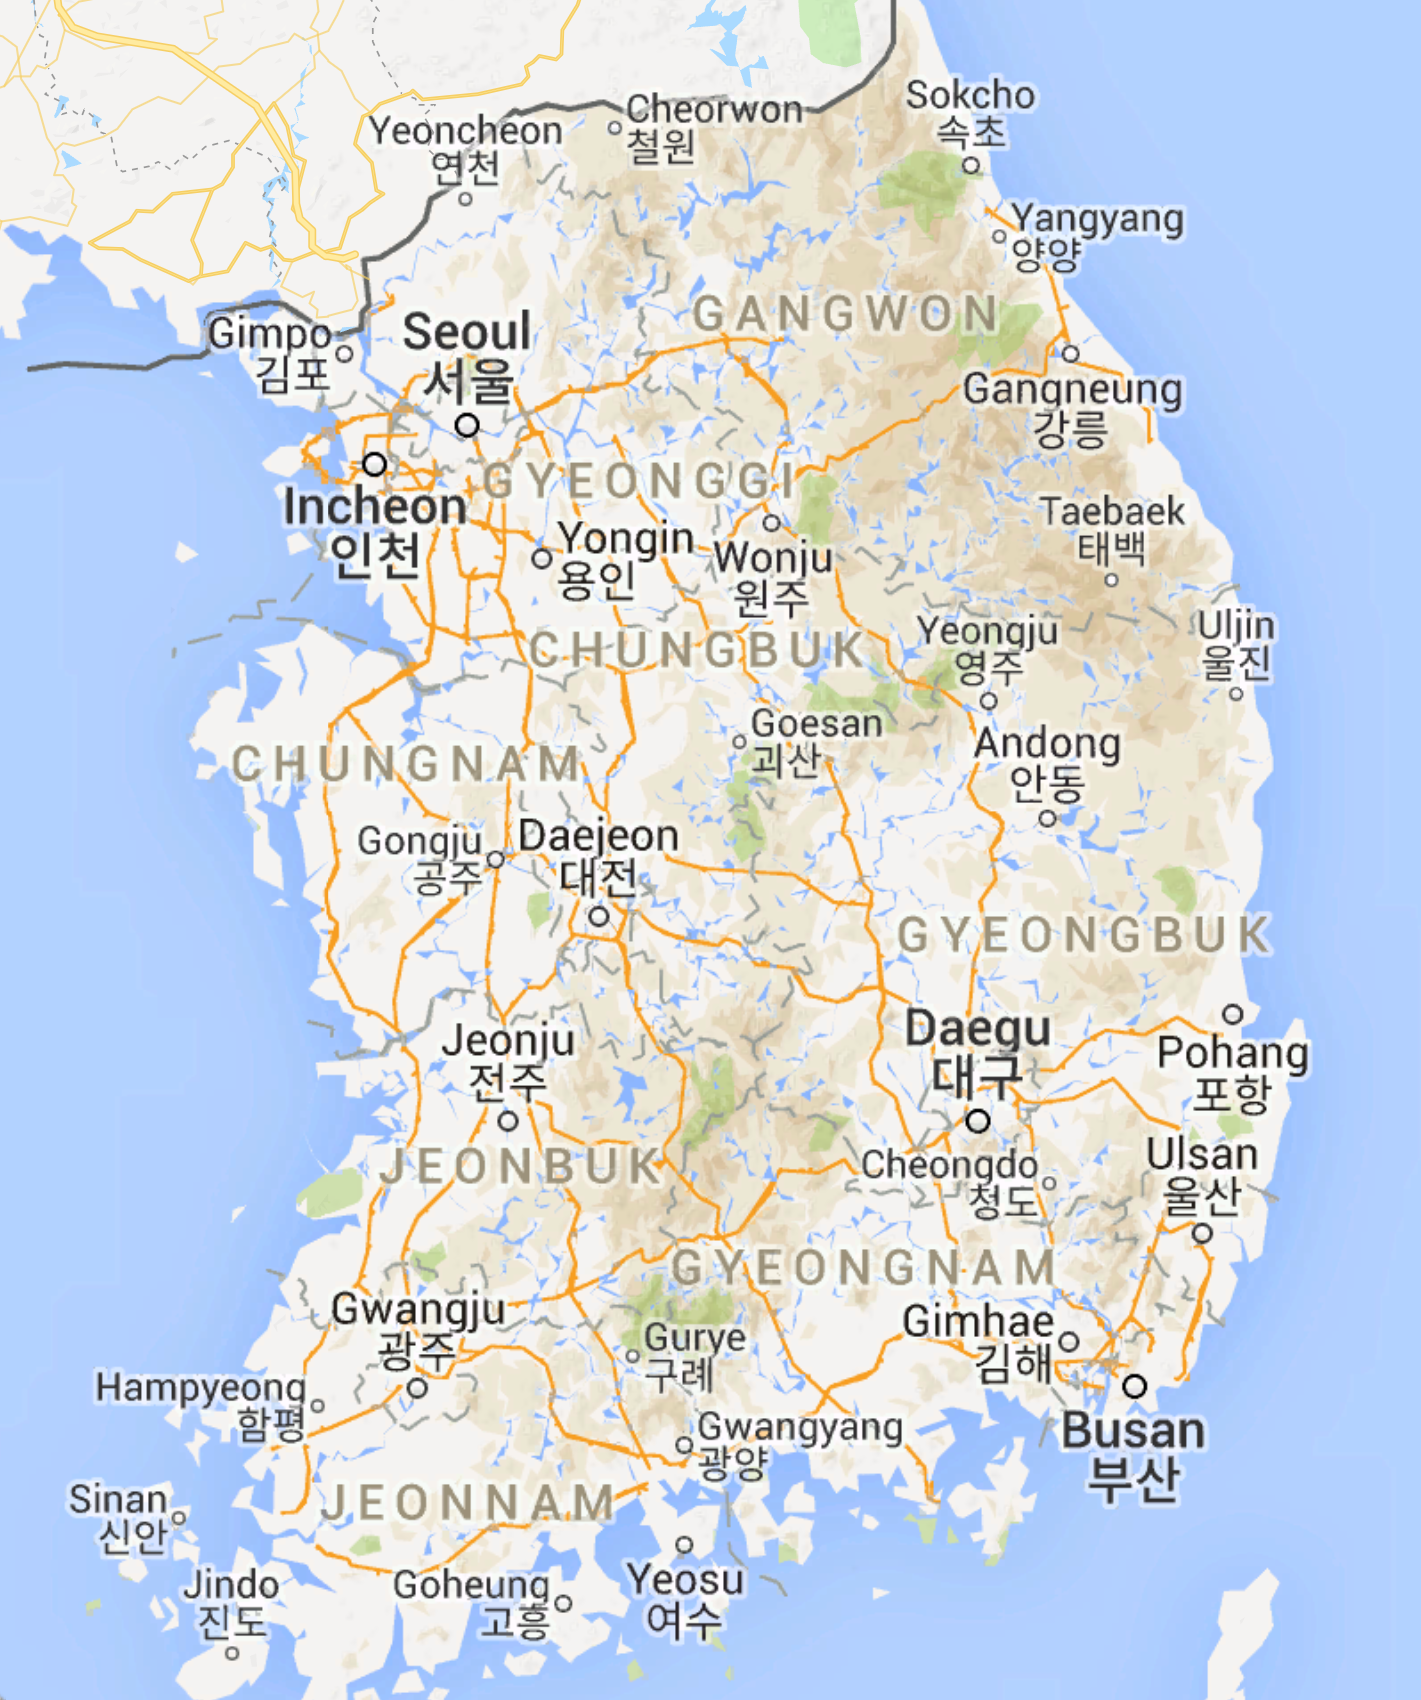
\includegraphics[width=14cm]{Korea.PNG}
\caption{South Korea} 
\end{figure}

\subsection{2A}

if Korea could migrate all their personal passenger vehicles to all-electric vehicles instantaneously (no transition time required), they will need more than 10000 charger station, basing on the vehical they have nowadays and the capcity of each stall.

the key factors that shaped the development of EV is the cost of charging EVs. 

\subsection{2B}

Whatever the number of elctric cars ,the country must have wide spread of charging stations. We should build a mix of both city-based chargers and  rural chargers. 

The superchargers should spread alone the highway ,while the terminal chargers should build near office center and hotel.

\subsection{2C}

The full evolution to electric vehicles in Korea may come ture in 2025.
the key factors that shaped proposed growth plan timeline is the tecnology that makes charge stations.


\section{Task 3}

China and Australia with very different geographies, population density distributions, and wealth distributions, may have different solutions.China has large amount of population ,the require for vehical is realy high ,so they will take,much more time.



\section{Task 4}

Nowadays, there emerge various high-tech transportation modes such as car-share and ride-share services, self-driving cars, rapid battery-swap stations for electric cars, and even flying cars and a Hyper-loop.

 The car-pooling service matches up car owners who are willing to offer a ride with those needing a lift, in the hope of making trips to their destination more convenient and cost-effective.Driver-less vehicles free driver’s hands and concentration.

Battery-swap stations for EV give rise to a more favourable charging experience. Flying cars take full advantage of space and together with Hyper-loops, it shortens travel time tremendously. 

Moreover, all of these technologies serving as alternatives to traditional transportation contribute to a superior allocation of transportation resources, alleviate the strain on public transport plus environment, and promote the transformation of global energy structure.

EVTOL (electric vertical take-off and landing aircraft) as the most promising solution for flying cars is faster than the EV. The EVTOL's demand of power is also very high. As more and more EVOTLs used, grid load will increase rapidly, we will need more powerful electric grid.In some big city that will be very crowd , EVTOL may take the place of EV.

\begin{figure}[htbp]
\small
\centering
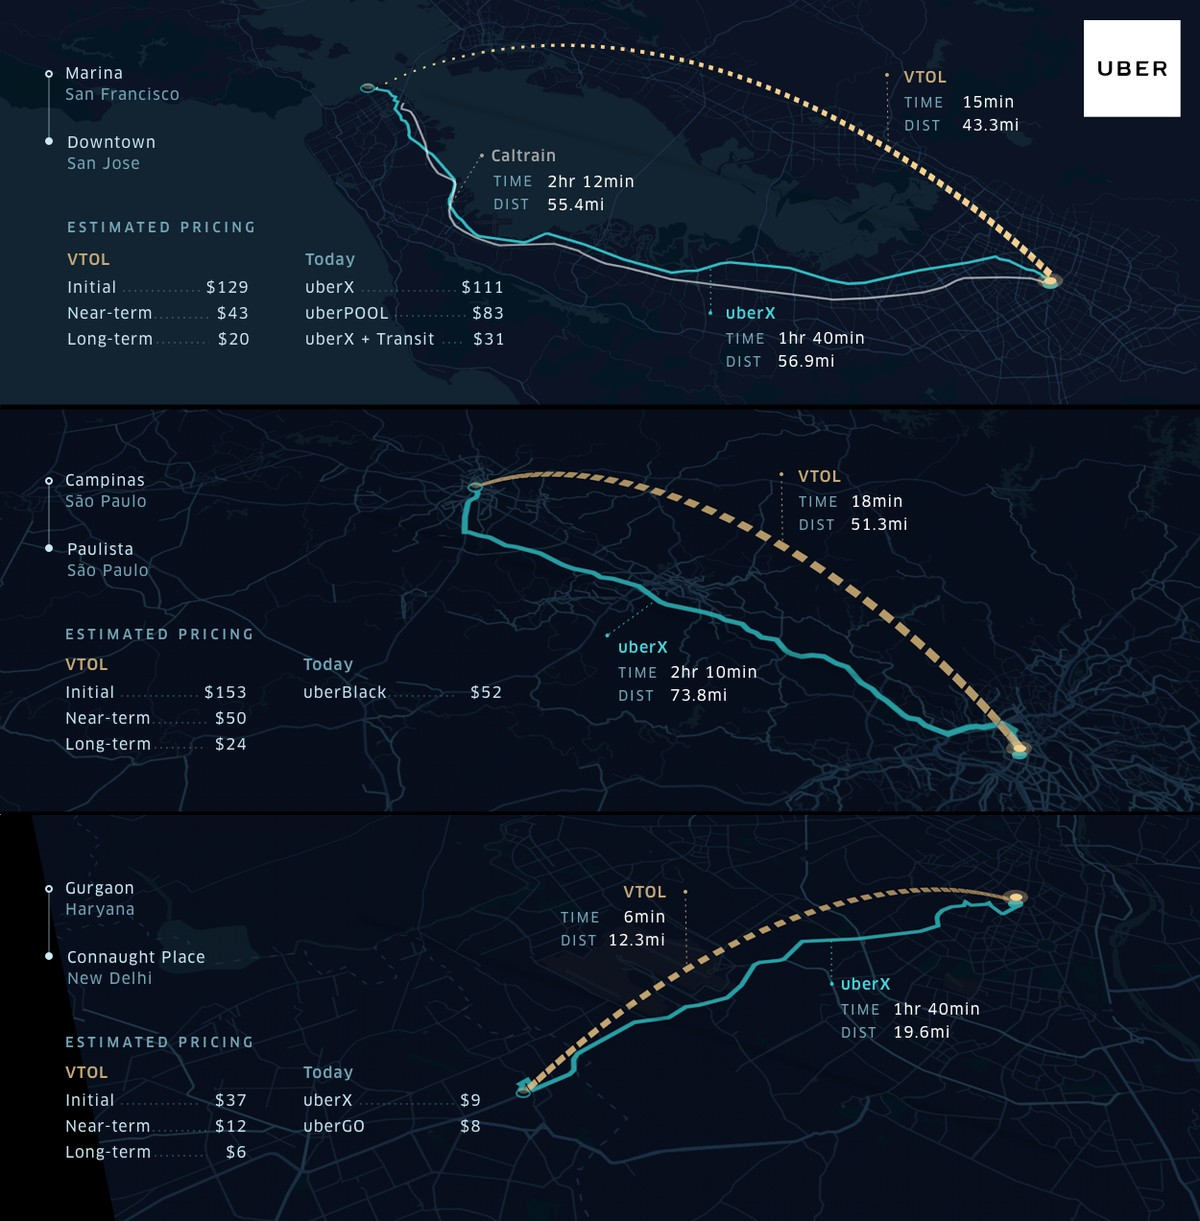
\includegraphics[width=16cm]{1.png}
\caption{EVTOL taxis and normal taxis} 
\end{figure}

Hyperloop is much more faster than any vehical we have nowadays, people will spend less time when travalling long distance, Hyperloop may play the role of train rather than the car. Also Hyperloop will use solarpower , personally, we think Hyperloop will have little affect on EV.

Car-share and ride-share services will reduce the price we pay. Rapid battery-swap stations for electric cars will facilitate people's lives. They will accelarate the speed of EV devolpment.

\newpage

\section{Task 5  The Handout} 

Distinguished leaders:

    It's my privilege to be here to illustrate the key factors you need to consider as you return to your motherland to develop a national plan to migrate personal transportation towards all-electric cars and set a gas vehicle-ban date. 
    
    From my perspective, the key factors are the price of Electric Vehicles, charging cost, the distribution of charging piles and the capacity of the grid. First, the price of Electric Vehicles and the charging cost restricts nationals' purchasing power and influences the acceptance of electric cars in the nationals thereby affecting the all-electric switch. 	
    
    Second, for the driving range of EVs is inevitably limited to some degree, the distribution of charging stations is closely connected to the degree of drivers' range anxiety, which is absolutely relevant to the implementation of personal EVs.
    
     Moreover, to carry out practical policies, leaders ought to take the capacity of the nation's grid into consideration, because the grid will definitely shoulder heavy burden due to the all-electric transition. 
     
     The factors I mentioned before are of primary importance to your policies as far as I'm concerned. 
     
     Thanks for your listening!


\newpage


\begin{thebibliography}{99}
\bibitem{1} D.~E. KNUTH   The \TeX{}book  the American
Mathematical Society and Addison-Wesley
Publishing Company , 1984-1986.
\bibitem{2}Lamport, Leslie,  \LaTeX{}: `` A Document Preparation System '',
Addison-Wesley Publishing Company, 1986.
\bibitem{3}\url{https://supercharge.info/}
\bibitem{4}\url{https://insideevsforum.com/}
\end{thebibliography}

\begin{appendices}

\section{First appendix}

Here are simulation programmes we used in our model as follow.\\

\textbf{\textcolor[rgb]{0.98,0.00,0.00}{Input matlab source:}}
\lstinputlisting[language=Matlab]{./code/SuperChargeStation.m}

\textbf{\textcolor[rgb]{0.98,0.00,0.00}{Input matlab source:}}
\lstinputlisting[language=Matlab]{./code/EVusage.m}

Here is the Rate simulation:\\

\textbf{\textcolor[rgb]{0.98,0.00,0.00}{Input matlab source:}}
\lstinputlisting[language=Matlab]{./code/Rate.m}

\section{The Voronoi Code And The Circle Code}

\textbf{\textcolor[rgb]{0.98,0.00,0.00}{Input matlab source:}}
\lstinputlisting[language=Matlab]{./code/Voronoi.m}

\textbf{\textcolor[rgb]{0.98,0.00,0.00}{Input matlab source:}}
\lstinputlisting[language=Matlab]{./code/circular.m}


\end{appendices}
\end{document}




%% 
%% This work consists of these files mcmthesis.dtx,
%%                                   figures/ and
%%                                   code/,
%% and the derived files             mcmthesis.cls,
%%                                   mcmthesis-demo.tex,
%%                                   README,
%%                                   LICENSE,
%%                                   mcmthesis.pdf and
%%                                   mcmthesis-demo.pdf.
%%
%% End of file `mcmthesis-demo.tex'.
